\begin{tikzpicture}
    \definecolor{red}{RGB}{219, 50, 54}
    \definecolor{yellow}{RGB}{244, 194, 13}
    \definecolor{blue}{RGB}{72, 133, 237}
    \definecolor{green}{RGB}{60, 186, 84}
    \definecolor{orange}{RGB}{230, 122, 22}
    \definecolor{purple}{RGB}{145, 91, 145}
    \definecolor{grey}{RGB}{211, 211, 211}
    
    \tikzstyle{a}=[thick, rounded corners]
    \tikzstyle{attention}=[thick, rounded corners, minimum width=4.5cm]
    
    \tikzmath {
        \imgSize = 1;
        \inputPad = 0.15;
    }
    
    \coordinate (input_bl) at (0,0);
    \coordinate (input_tr) at ($(\imgSize * 2 + \inputPad * 3, \imgSize * 2 + \inputPad * 3 + 0.5)$);
    \coordinate (input_cr) at ($(\imgSize * 2 + \inputPad * 3, \imgSize + \inputPad * 1.5 + 0.25)$);
    
    \draw[thick, rounded corners] (input_bl) rectangle (input_tr);
    
    \coordinate (input1_c) at ($(input_bl) + (\inputPad + \imgSize / 2, \inputPad + \imgSize / 2)$);
    \node[inner sep=0pt] (input1) at (input1_c) {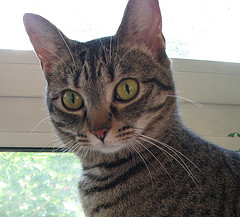
\includegraphics[width=1cm]{figures/cat1.png}};
    
    \coordinate (input2_c) at ($(input_bl) + (2*\inputPad + \imgSize * 1.5, \inputPad + \imgSize / 2)$);
    \node[inner sep=0pt] (input2) at (input2_c) {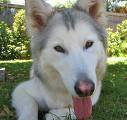
\includegraphics[width=1cm]{figures/dog.png}};
    
    \coordinate (input3_c) at ($(input_bl) + (\inputPad + \imgSize / 2, 2*\inputPad + \imgSize * 1.5)$);
    \node[inner sep=0pt] (input3) at (input3_c) {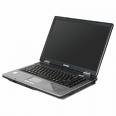
\includegraphics[width=1cm]{figures/laptop.png}};
    
    \coordinate (input4_c) at ($(input_bl) + (2*\inputPad + \imgSize * 1.5, 2*\inputPad + \imgSize * 1.5)$);
    \node[inner sep=0pt] (input4) at (input4_c) {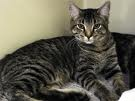
\includegraphics[width=1cm]{figures/cat2.png}};
    
    \coordinate (input_txt_c) at ($(input_bl) + (\inputPad * 1.5 + \imgSize, 3*\inputPad + 2*\imgSize + 0.1)$);
    \node[] (input_txt) at (input_txt_c) {Inputs};
    
    \coordinate (encoder_c) at ($(input_cr) + (2, 0)$);
    \node[draw, thick, inner sep=0.25cm, align=center, rounded corners, fill=blue!50] (encoder) at (encoder_c) {Encoder \\ Network};
    
    \coordinate (output_cl) at ($(encoder_c) + (2, 0)$);
    \coordinate (output_similar_bl) at ($(output_cl) + (0,0.125)$);
    \coordinate (output_similar_cl) at ($(output_similar_bl) + (0, \imgSize / 2 + \inputPad)$);
    \coordinate (output_similar_tr) at ($(output_similar_bl) + (2 * \imgSize + \inputPad * 3, \imgSize + 2 * \inputPad)$);
    \draw[thick, rounded corners, color=green] (output_similar_bl) rectangle (output_similar_tr);
    
    \coordinate (output_similar1_c) at ($(output_similar_bl) + (\inputPad + \imgSize / 2, \inputPad + \imgSize / 2)$);
    \node[inner sep=0pt] (output_similar1) at (output_similar1_c) {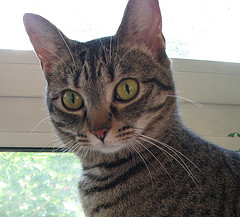
\includegraphics[width=1cm]{figures/cat1.png}};
    
    \coordinate (output_similar2_c) at ($(output_similar_bl) + (2*\inputPad + \imgSize * 1.5, \inputPad + \imgSize / 2)$);
    \node[inner sep=0pt] (output_similar2) at (output_similar2_c) {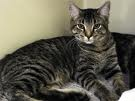
\includegraphics[width=1cm]{figures/cat2.png}};
    
    \coordinate (text_similar_c) at ($(output_similar_tr) + (0.25, -\imgSize / 2 - \inputPad)$);
    \node[anchor=west, color=green] at (text_similar_c) {Similar};
    
    \coordinate (output_unsimilar_bl) at ($(output_cl) - (0,0.125 + \imgSize + 2 * \inputPad)$);
    \coordinate (output_unsimilar_cl) at ($(output_unsimilar_bl) + (0, \imgSize / 2 + \inputPad)$);
    \coordinate (output_unsimilar_tr) at ($(output_unsimilar_bl) + (2 * \imgSize + \inputPad * 3, \imgSize + 2 * \inputPad)$);
    \draw[thick, rounded corners, color=red] (output_unsimilar_bl) rectangle (output_unsimilar_tr);
    
    \coordinate (output_unsimilar1_c) at ($(output_unsimilar_bl) + (\inputPad + \imgSize / 2, \inputPad + \imgSize / 2)$);
    \node[inner sep=0pt] (output_unsimilar1) at (output_unsimilar1_c) {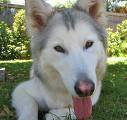
\includegraphics[width=1cm]{figures/dog.png}};
    
    \coordinate (output_unsimilar2_c) at ($(output_unsimilar_bl) + (2*\inputPad + \imgSize * 1.5, \inputPad + \imgSize / 2)$);
    \node[inner sep=0pt] (output_unsimilar2) at (output_unsimilar2_c) {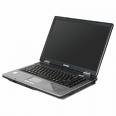
\includegraphics[width=1cm]{figures/laptop.png}};
    
    \coordinate (text_unsimilar_c) at ($(output_unsimilar_tr) + (0.25, -\imgSize / 2 - \inputPad)$);
    \node[anchor=west, color=red] at (text_unsimilar_c) {Not Similar};
    
    \draw[thick, ->] (input_cr) -- (encoder);
    \draw[thick, ->] (encoder.east) -- (output_similar_cl);
    \draw[thick, ->] (encoder.east) -- (output_unsimilar_cl);
    

\end{tikzpicture}